\documentclass[10pt,letterpaper]{article}
\usepackage[latin1]{inputenc}
\usepackage{amsmath}
\usepackage{amsfonts}
\usepackage{amssymb}
\usepackage{graphicx}

\DeclareMathOperator*{\argmax}{arg\,max}

\author{Sarun Gulyanon}
\title{3D Neuron Pose Estimation from Calcium Image Stack Sequences Using Neuron Plane Model}
\begin{document}

\maketitle

\section{Abstract}
It is known that the sensory neurons control the locomotion but we do not know how this happens. The lack of robust tools for simultaneous quantification of both morphology and neuronal activity in calcium images hinders the progress. The main issues are that these calcium images are noisy, have low resolution in Z-axis, contain significant deformations of neurons, and suffer from characteristics of calcium images. In this work, we developed the semi-automatic approach for robust 3D pose estimation of neurons. It requires little user intervention to aid with dendrite detection. Then, our method incorporates the image appearance, local and global shape, as well as domain knowledge about neuron morphology, to find the best fitting neuron configuration to the input data using our neuron plane model. We validated our results using time-lapse calcium image stacks of larval Drosophila sensory neuron.
%In our experiments we illustrate how our method can track neurites under severe local intensity ambiguities.
%Calcium image are noisy but it give key information in understanding the relationship between morphology and functionality of neurons. However, the large amount of data must be processed to reveal this relationship so the manual approach is infeasible. To quantify both properties, we need to track neurons over calcium image sequences. Due to noise, only 2D image is reliable for quantification; however, the 3D neuron configuration is of interest. So we develop the semi-automatic method to estimate the 3D configuration of neuron morphology from 2D calcium image sequences. To make the problem feasible, With our hypothesis on the model of neuron, we enforce it along with  

\section{Introduction}
% why we want to study the link between locomotion and neuron activity
Over decades, we know that sensory neurons control the locomotion process but we poorly understand the molecular mechanisms that determine the responses of the proprioceptive cells. To answer this question, we use high speed confocal microscopy to describe how the dendrites of proprioceptive neurons in larval Drosophila are deformed by the forces of crawling motions. Surprisingly, the pattern of deformation for a given neuron is unique in each direction of motion \cite{Gulyanon2018a}; and two particular neurons (dda-D and dda-E) show strong activation level during the locomotion. To gain insight into the underlying mechanisms, we must expose the link between the change in morphology due to the locomotion and the neuronal activity of the neuron pair.

% why do we need to analyze the calcium images
Fortunately, calcium imaging holds the key to understanding the relationship between neuron morphology and neuronal activity because its intensity is proportional to the neuronal firing level; as a result calcium images also show the location of active regions in neurons. Hence, the time-lapse calcium imagery allows us to observe both neuron morphology and neuronal activity simultaneously in larva Drosophila. Due to the large amount of image sequences required for learning the link between locomotion and sensory neuron activity, the manual approach is infeasible; and the lack of robust tools for simultaneous quantification of both morphology and neuron activity hinders the progress.

% challenge
The quantification of neuronal morphology is tricky due to four reasons. First, it involves tracking neurons in 3D over noisy calcium image sequences. Second, time-lapse image stacks have low resolution in Z-axis due to the limitation of imaging system. Third, the deformation of neurons during the locomotion compromises the slices of image stack sequences. Moreover, the deformation can be severe and creates a large displacement. Last, the most challenging problem is the characteristics of calcium images, which has low intensity when neurons are inactive so the neurons are barely visible in such cases. And they have high intensity when they are active but they are usually deformed in those frames as well (fig.~\ref{fig:calcium_img}).

\begin{figure}
	\centering
	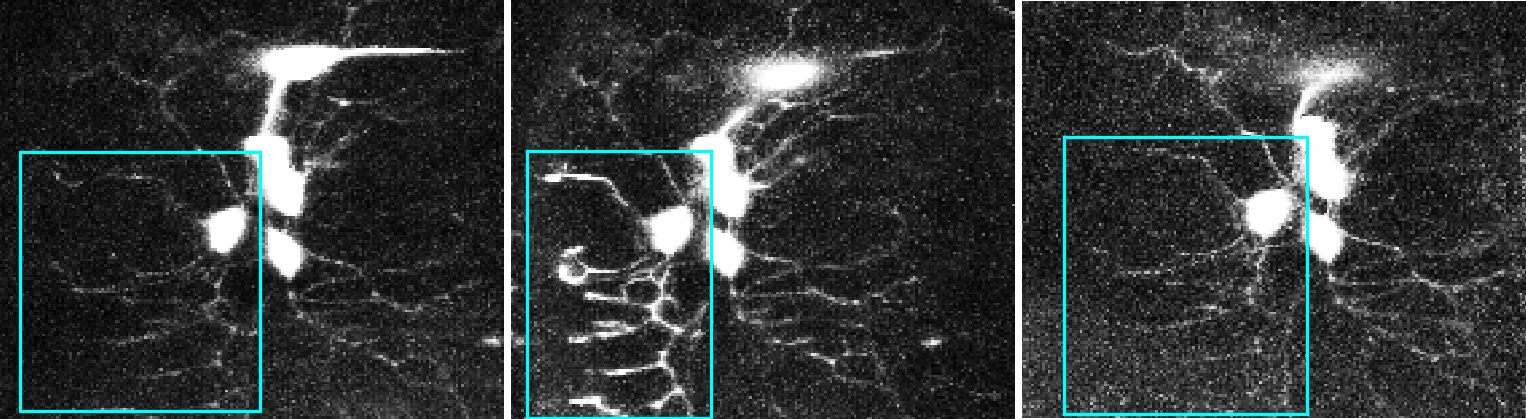
\includegraphics[width=0.7\linewidth]{img/calcium_img}
	\caption{Calcium image characteristics. Frames in temporal order of the same neuron (cyan boxes). First and last frames are when neurons are inactive so they are dim. Middle is active neuron. Although it is bright but it is deforming as well. Intensity is adjusted for visualization purposes.}
	\label{fig:calcium_img}
\end{figure}

% our approach: overview
Here we developed the semi-automatic 3D neuron pose estimation method that can handle these issues and helps reduce the operation time in quantifying both the morphology and neuron activity. It requires little user interaction, including the initial trace and the location of the farthest tips of dendrites, to help handle tracking issues. Then, our method finds the best fits neuron configuration by fitting the neuron plane model based on the image feature, neuron local and global shape, and the domain knowledge about the deformation during the crawling locomotion. Finally, the deformed traces are efficiently recovered using the neuron plane model.


\section{Method}
% motivation of using neuron plane model
First we present the neuron plane model, which is a simplified representation of the neuron pairs. It helps reduce the number of parameters required for describing the deformation of neurons over the image sequences. 


\subsection{Neuron Plane Model}
% issue with previous method : neuron tree structure model
% assumption 1: reduce DoF
The main issue of neuron tree structure is that it has high degree of freedom (DoF) and there are insufficient number of constraints to find the acceptable results. To make this problem feasible, first we assume that neuron mass is preserved and it is enclosed by the surface (the skin or epidermis of Drosophila larvae). So we can model the deformation of the neuron through the deformation of the enclosing surface.
% assumption 2: reduce number of possible states
Second, we limit the direction of crawling locomotion of samples. Drosophila larvae are observed by putting the samples through a tiny channel to prevent the larvae from moving into another direction except for forward or backward. As a result, we need to model the deformation only in one direction (X-axis).

% definition
With these assumptions, we define the neuron plane model enclosing the neuron pair at time $t$ as the linear chain model of pictorial structures \cite{Felzenszwalb2005} consisting of $2N$ equal-width stripes/parts, ${\bf S}^t = \{s_i^t\}$, for $i = 1,...,2N$ and $t = 0,...,T$ (fig.~\ref{fig:planemodel}). A set of part parameter $\theta^t = \{\theta_i^t\}$ indicating the orientation in XZ-axis at time $t$ (we assume there are no movements in Y-axis). $L(s_i^t)$ and $R(s_i^t)$ are the functions indicating the leftmost and rightmost locations of the stripe $s_i^t$ respectively. To standardize the neuron plane model, the middle line of the neuron plane model $R(s_N^t)$, $L(s_{N+1}^t)$ lies between the two soma of a neuron pair. The centroid of soma is detected using the circular Hough transform \cite{Duda1972}.

\begin{figure}
	\centering
	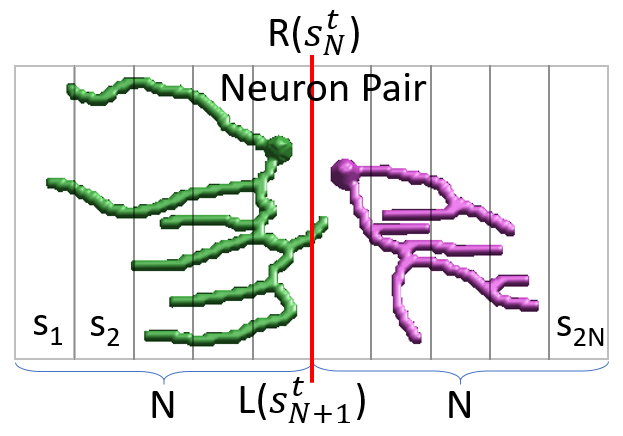
\includegraphics[width=0.4\linewidth]{img/plane_model}
	\caption{Neuron plane model of a neuron pair (green and magenta) split the bounding box into $2N$ stripes. Its middle line (red line), $L(s_{N+1}^t)$ and $R(s_N^t)$, aligns with the center between soma.}
	\label{fig:planemodel}
\end{figure}


\subsection{Optimization}
Calcium image characteristics makes it challenging to get reliable tracking results in every frame (fig.~\ref{fig:calcium_img}). To tackle this difficulty, our method requires user interaction, including the initial trace, $Y^0$, when the neuron pair is flat and the X-coordinate of the farthest dendrite tips at time $t$, $p^t_k$ (fig.~\ref{fig:ui}). To convert the initial trace $Y^0$ to the plane model, the number of parts $N$ is picked to be just high enough to enclose the trace and $\theta_i^0 = 0$.

Given the volume sequence $V = \{V^t\}$, we formulate the objective function as the conditional distribution over the neuron plane model at time $t$, $\theta^t$:
\begin{equation}
\hat{\theta}^t = \argmax_{\theta^t} P(\theta^t | V^t, \theta^{t-1}, p^t_k) = \exp \left\{ - \sum_{t=1}^T \left( E_{x}(\theta^t,V^t, p^t_k) + E_{z}(\theta^t,\theta^{t-1}) \right) \right\}
\end{equation}

Although using neuron plane model improves the efficiency in finding the optimal trace configuration $Y^t$ because it has lower number of DoF, we improve its efficiency further by dividing the optimization into two steps --- X-optimization (Sec.~\ref{sec:x-optim}) and Z-optimization (Sec.~\ref{sec:z-optim}), in order to achieve lower latency. Both steps are optimized using the simulated annealing technique \cite{Kirkpatrick1983}.

\begin{figure}
	\centering
	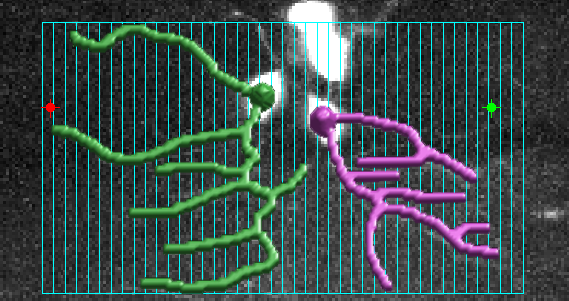
\includegraphics[height=70pt]{img/user_ui}
	\quad
	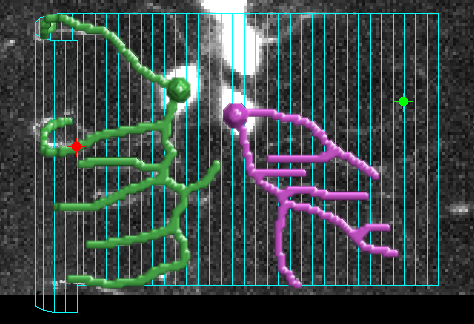
\includegraphics[height=70pt]{img/user_ui13}
	\caption{User interaction at two frames, $t=\{0,12\}$, respectively. Red and green points are the X-coordinates of the farthest dendrite tips and the initial traces of a neuron pair in magenta and green. The corresponding neuron plane model in cyan color.}
	\label{fig:ui}
\end{figure}


\subsubsection{X-Optimization} \label{sec:x-optim}
This step finds the neuron plane configuration in X-axis, $\theta_i^t \in \{0, \pi/8, \pi/4, 3\pi/8 \}$, that best match to the input data, while enforcing the constraints of smooth flat surface.
\begin{equation}
E_{x}(\theta^t,V^t,p^t_k) = E_{img}(\theta^t,V^t) + E_{shape}(\theta^t) + E_{flat}(\theta^t) + E_{con}(\theta^t, p^t_k)
\end{equation} 

\paragraph{Image feature} term $E_{img}$ selects the neuron plane configuration that maximizes the normalized cross correlation \cite{Yoo2009} between the first frame, $V^0$, cropped around the neuron pair and the transformed frame, $T(V^t, \theta^t)$, with respect to the neuron plane model (Section~\ref{sec:gettrace}). Since the calcium image stacks are noisy, the maximum projection of image stacks, $I^t$, are preferred to make the input images more reliable. 
\begin{equation} \label{eq:Eimg}
E_{img}(\theta^t,I^t) = NCC(I^t, T(I^0, \theta^t))
\end{equation} 

\paragraph{Shape energy} term $E_{shape}$ enforces the smoothness over the orientation parameters of the neuron plane model.
%  is the term that encourage similar orientation between adjacent parts.
\begin{equation}
E_{shape}(\theta^t) = \sum_{i=1}^{2N-1} (\theta_{i+1}^t - \theta_i^t)^2
\end{equation} 

\paragraph{Flat surface energy} term $E_{flat}$ encourages flat surface to capture the whole neurons when they start folding.
\begin{equation}
E_{flat}(\theta^t) = \sum_{i=1}^{2N} (\theta_i^t)^2
\end{equation} 

\paragraph{Constraint energy} term $E_{con}$ matches the dendrites tips derived from the neuron plane model with the user-given ones. 
\begin{equation} \label{eq:Econ}
E_{con}(\theta^t, p^t_k) = \sum_{k=1}^{2} (p_k^t - T(p_k^0, \theta^t))^2
\end{equation} 

%Given the neuron trace in one frame at the stationary state. 
%Here we presentation the plane with a number of stripes and the parameters are the angle between adjacent stripes. This is possible because of the assumption we made.

%First we fit the neuron in the next time step in 2D. Using the rotation to limit the degree of freedom.


%To make it feasible, we model the rotation only in X-axis. This is possible because of how the calcium image sequences are taken. Since the crawling movement of Drosophila larva is observed by putting the sample through an tiny channel to prevent the larva from moving into another direction except forward or backward. Therefore, we can model only in one direction.

\subsubsection{Z-Optimization} \label{sec:z-optim}
The second optimization finds the configuration that match our neuron model, whose main features includes smooth transition, low curvature, and low depth. The possible $\theta_i^t$ value at this stage is the reflection across the XY-plane. And this step is computed in post-processing since it requires no user input.
\begin{equation}
E_{z}(\theta^t,\theta^{t-1}) = E_{dep}(\theta^t) + E_{curv}(\theta^t) + E_{tran}(\theta^t,\theta^{t-1})
\end{equation}

\paragraph{Depth energy} term $E_{dep}$ adjusts the plane to have low depth, since we observed that dendrites always appear over 5-10 slices ($?? \mu m$) %% Ask Liping
\begin{equation}
E_{dep}(\theta^t) = \sum_{i=1}^{2N} \left( D(\theta_i^t) \right)^2
\end{equation} 
where $D(\theta_i^t)$ is the depth of the part $i$ at time $t$.

\paragraph{Curvature energy} term $E_{curv}$ encourages low curvature configuration to regularize the neuron plane model.
\begin{equation}
E_{curv}(\theta^t) = \sum_{i=2}^{2N-1} (R(s_{i+1}^t) - 2L(s_i^t) + L(s_{i-1}^t))^2
\end{equation} 

\paragraph{Transition energy} term $E_{tran}$ enforces smooth transition between adjacent time steps.
\begin{equation}
E_{tran}(\theta^t) = \sum_{i=1}^{2N} \left\{ D(\theta_i^{t-1}) - D(\theta_i^t) \right\}^2
\end{equation}


\subsection{Retrieving Deformed Traces} \label{sec:gettrace}
%To recover the deformed neuron traces using the neuron plane model.
The neuron plane model represents the deformation of the initial trace via the uniform cubic B-spline
free-form deformations (FFD) \cite{Rueckert1999}. To recover the deformed neuron traces $Y^t$, first we need to get the control points ${\bf C}^t = \{c_k^t\}$, which is defined by endpoints of parts.
%we apply free-form deformation (FFD) \cite{Rueckert1999} on the initial trace, where the control points of ffd is defined by the stripes of neuron plane model. The transformation of the initial neuron trace is defined by the neuron plane model as following.
\begin{equation}
c_k^t = 
\begin{cases}
L(s_{k+1}^t), & \text{if } 0 \leq k \leq N-1 \\
R(s_k^t), & \text{if } N \leq k \leq 2N \\
\end{cases}
\end{equation}

Then, the transformation $T({\bf x}, \theta^t)$ at any point ${\bf x} = (x,y,z)$ is defined as,
\begin{equation}
T({\bf x}, \theta^t) = \sum_{c_k^t \in {\bf C}^t} \eta({\bf x}, c_k^t) {\bf d}_k^t
\end{equation}
where $\eta$ is the coefficient of the control point $c_k^t$ with displacement ${\bf d}_k^t = c_k^t - c_k^0$ at point ${\bf x}$.




%Recovering Trace from Neuron Plane Model
%After we get the neuron plane model, we apply free-form deformation (FFD) \cite{Rueckert1999} on the initial trace, where the control points of ffd is defined by the stripes of neuron plane model. The transformation of the initial neuron trace is defined by the neuron plane model as following.

%The same step can be applied to the image patches or points in eqs.\eqref{eq:Eimg} or \eqref{eq:Econ}.


\section{Experiments}
% dataset overview
We validated our method on the time-lapse calcium volumes dataset of larval Drosophila sensory neurons. Larvae expressing the genetically encoded calcium sensor GCaMP6.0F in the proprioceptors were observed in four dimensional confocal microscopy imagery. This is achievable because the neurons are found directly beneath the cuticle and epidermis which are optically transparent.

% dataset detail and metric
In this dataset, each sequence captured the neuronal displacements and deformations during crawling locomotion over 10-50 frames. We measure how well model fits the data using the mutual information (MI) \cite{Viola1997} between artificial volume produced by the deformed initial traces against the input volumes. MI is defined by, $MI(A,B) = \sum_{a \in A}\sum_{b \in B} P(a,b) \log \frac{P(a,b)}{P(a)P(b)}$, where $A$ is the input volume and $B$ is the artificial volume derived from the neuron plane model. Maximizing the mutual information find the best aligned volumes.

% significance of each component
We are the first method for recovering 3D neuron pose from calcium image sequences. Previous works \cite{Ferrari2009, Glowacki2017} in pose estimations are incapable of handling issues in noisy time-lapse calcium volumes during the locomotion. Table~\ref{tab:result} emphasizes the significance of two novel components, $E_{dep}$ and $E_{flat}$, in our energy function formulation or lack thereof. The depth energy is required to bound the thickness of neurons (fig.~\ref{fig:Edep}). Although the resolution of image stacks in Z-axis is low, the thickness of neurons can still be approximated and it shows that neurons have low thickness. The flat surface energy encourages the plane to fold rather than squeeze the neurons to fit the input volume. (fig.~\ref{fig:Eflat}) 


\begin{figure}
	\centering
	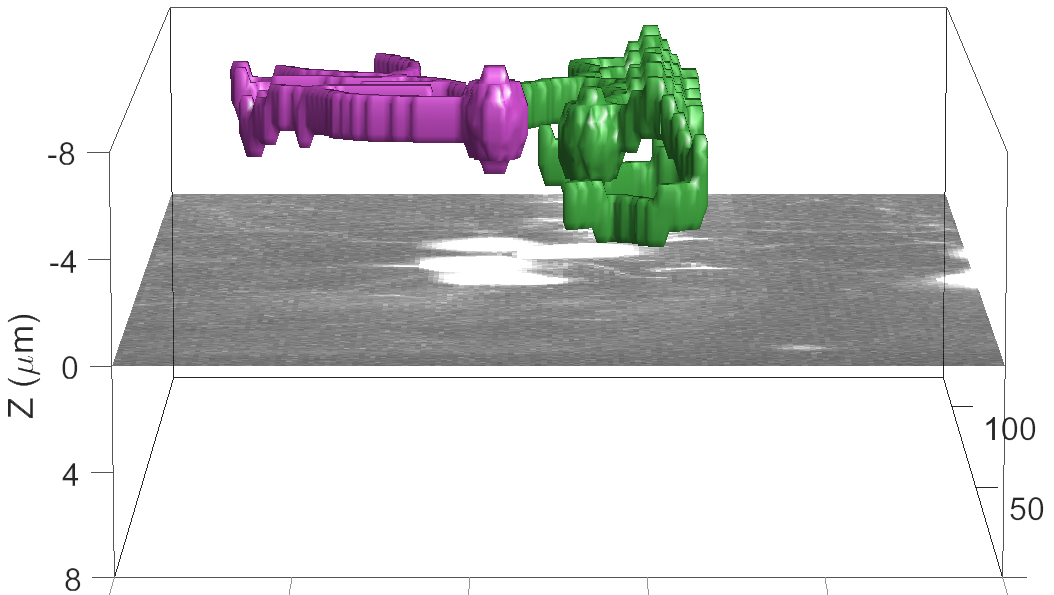
\includegraphics[height=80pt]{img/norm2}
	~
	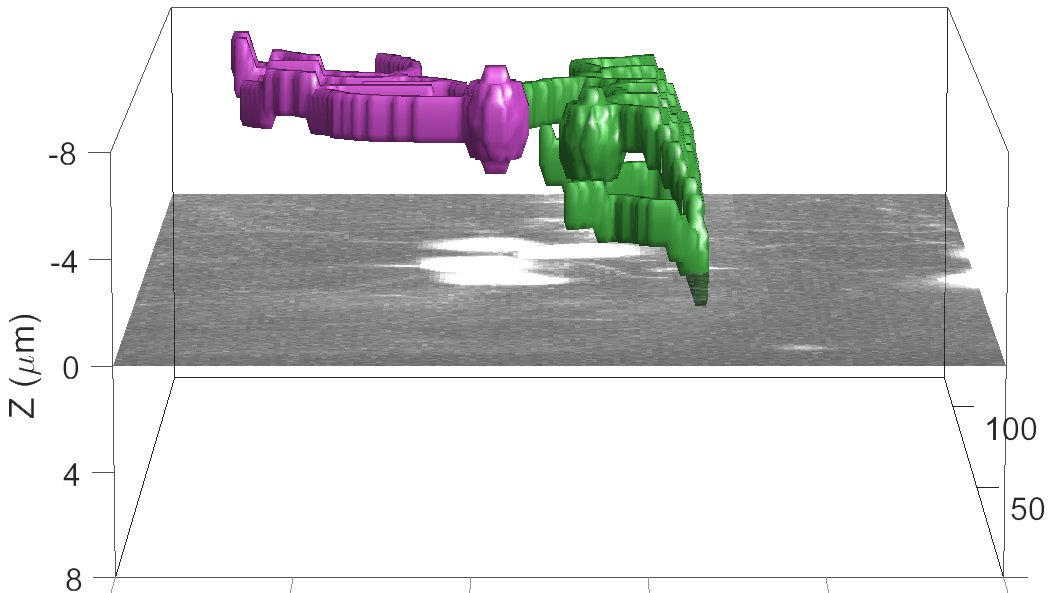
\includegraphics[height=80pt]{img/dep2}
	\caption{The importance of depth energy $E_{dep}$ that limits the depth of traces (left) within the image stack (9 slices, $z=0,...,8$ in this example). Otherwise, the depth may be overestimated and higher than the thickness of the image stack (right).}
	\label{fig:Edep}
\end{figure}

\begin{figure}
	\centering
	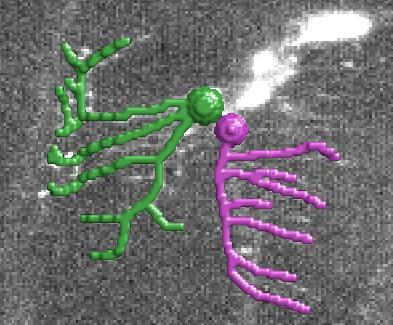
\includegraphics[height=80pt]{img/norm1}
	~
	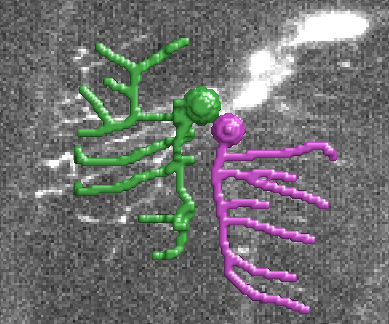
\includegraphics[height=80pt]{img/flat1}
	\caption{The importance of flat surface energy $E_{flat}$. It encourages the neuron plane to fold (left) instead of squeezing it to fit the input volume (right).}
	\label{fig:Eflat}
\end{figure}





\begin{table}[b]
	\centering
	\begin{tabular}{|c|c|c|c|}
		\hline 
		& Our Method & $E_{dep} = 0$ & $E_{flat} = 0$ \\ 
		\hline 
		Avg & 0.1446 & 0.1380 & 0.1436 \\ \hline
		Std & 0.0342 & 0.0330 & 0.0340 \\
		\hline 
	\end{tabular}
	\caption{The mutual information similarity results between the artificial trace volume produced from the neuron plane model against the input volumes. From left to right: our model, our model without the depth energy term, and our model without the flat surface energy term. The rows show the average and the standard deviation over the volume sequences.}
	\label{tab:result}
\end{table}


% faster when we separate the optimization
Second, we show the improvement in computation compared to when these two optimization is combined. The reason that we need to perform two estimations are purely for efficiency. Since this is the semi-automatic method so the performance in term of efficiency is very important in order to provide quick response time. In the experiments, we achieve the average speed around 15 FPS on mid-end computer (Intel Core i7-5500U CPU 2.40 GHz DDR3 8.00GB). If we combines the two steps we end up with around 3FPS. The efficiency gain comes from the separation of user-involved process and automatic process.


\section{Conclusion}
%Each component incorporate different factors, i.e., image features, local and global shape of neurons, and domain knowledge about the deformation. These two optimization steps could be merged into one step but we break it down into two purely for improving efficiency.

We presented the semi-automated 3D neuron pose estimation method via neuron plane model for calcium volume sequences. Our method incorporates the image feature, neuron local and global shape characteristics, and the domain knowledge about the deformation during the crawling locomotion. Our neuron plane model enclosing the neuron pair offers a simplified model. While breaking down the optimization into two steps helps reduces latency to user interactions. Our method is robust to noisy calcium volumes with severe deformations and requires only little user interaction. We validated our results using the time-lapse calcium volumes dataset of larval Drosophila sensory neurons.

\bibliographystyle{unsrt}
\bibliography{all}
\end{document}